\chapter{Weak Galerkin Parallel Solutions of Linear Elasticity on Unstructured Meshes}

This chapter focuses on solving linear elasticity problem on parallel computer by combining a novel finite element method with an efficient parallel computing scheme. Specifically, this combination involves a discontinuous weak Galerkin finite element method \cite{mu2012weak, li2013weak, wang2014weak, mu2013computational} and a non-overlapping domain decomposition scheme, namely, the balancing domain decomposition with constraints (BDDC) \cite{dohrmann2003preconditioner,tu2007three2d,tu2007three3d}. The WG method is considered as a newly developed robust numerical method and inherits the locking-free feature for the linear elastic equation \cite{wang2016locking}. 

Like the standard Finite Element method (FEM), the WG method can be used to solve generic partial differential equations. An advanced feature of the WG finite element method is that the entire problem is decomposed into multiple elemental problems. Such elemental problems are often derived from weak formulations of the corresponding differential operators after integration by parts. In these elemental problems, the differential operators are approximated and reconstructed by smaller-size matrices. The WG method has been proven robust and possessing optimal orders of accuracy in spatial discretization on serial computers \cite{mu2014weak, Mu2015new}. Wang et al \cite{wang2016locking} recently extended the WG method to solve linear elasticity problems and also successfully demonstrated its locking-free property. However, the performance of the WG method on parallel computers has not yet been examined.



\section{Domain Decomposition Scheme}
The basic idea of domain decomposition is to split the computational mesh of an entire domain into many smaller meshes for a set of non-overlapping subdomains. Each subdomain contains its own set of grid elements. For finite element methods, after domain decomposition, a remaining challenging task is to connect these subdomains' interfaces by satisfying continuity constraints to correctly represent the solution of the original set of equations over the complete domain. In this work, the BDDC method is used to serve this purpose. The original balancing domain decomposition (BDD) method \cite{mandel1993balancing} has only considered two level meshes. It used a multiplicative coarse domain to correct the local fine mesh subdomain. However, the significant difference between BDDC and BDD is that the method in this paper applies the coarse problem in an additive routine rather than multiplicative manner. In this case, a more flexible of constraints will reduce the complexity and improve the efficiency. In our BDDC method, we assemble the preconditioner matrix additively in contrast to the multiplicative coarse grid correction used in the BDD method. In the BDDC method, the flexibility of choosing constraining points leads to reduced complexity of implementation and improved efficiency of computations in comparison to the standard BDD method. The details of the choice of constraints for BDDC will be discussed in this section.

\subsection{FETI-DP Method}
Finite Element Tearing and Interconnect (FETI) , first proposed by Farhat\cite{farhat1991method, farhat1994optimal, klawonn2001feti, farhat1998two, li2006feti, klawonn2006dual}, is an iterative method for solving large finite element problems generated by linear equations. Originally, FETI is proposed to solve the discontinuity when apply domain decomposition on second order elliptic partial differential equations, particularly linear elasticity equations. FETI method partitioned the entire computational domain into two level meshes, the coarse grid and fine grid. Lagrangian multiplier is employed to conquer the discontinuity between each subdomain. For the fine mesh, since local matrix is not positive definite, the pseudo-inverse is applied to convert local matrix. 

Then FETI-DP (Dual Primal) is introduced for two-dimensional problems by Farhat and Rixen\cite{farhat2001feti}. In this new method, the unknown variables along the interface is partitioned into primal and dual spaces. The continuity of the primal unknown variables along the interface, the vertices of each subdomain, is maintained by assemblage. For the rest dual spaces, the constrains are still controlled by Lagrange multipliers. However, this constrain is only at the convergence of the method.

In this section, we begin with an example of a two-dimensional, two partitioned subdomain case. We enforce the Dirichlet boundary condition on the boundary. The original geometry and computational domain is  

\begin{figure}[h]
	\centering
	\begin{tabular}{c}
		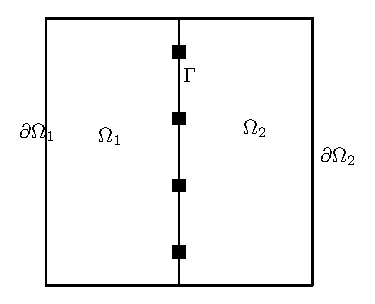
\includegraphics[width=0.6\textwidth]{./pics/feti1}
	\end{tabular}
	\caption{\footnotesize Computational domain partitioned into two nonoverlapping subdomains}\label{fig4: feti1}
\end{figure}

the original governing equation in matrix form is $ \mathbf{A} \mathbf{u} = \mathbf{f} $. We begin to compute the stiffness matrix for each subdomain that

\begin{equation}
 \begin{pmatrix}
A_{II}^{(j)} & A_{I\Gamma}^{(j)} \\
A_{\Gamma I}^{(j)} & A_{\Gamma \Gamma}^{(j)}
\end{pmatrix} \begin{pmatrix}
u_{I}^{(j)} \\ u_{\Gamma}^{(j)}
\end{pmatrix} = \begin{pmatrix}
f_{I}^{(j)} \\ f_{\Gamma}^{(j)}
\end{pmatrix}
\end{equation}
\subsection{Balancing Domain Decomposition by Constraints}

The balancing domain decomposition method was introduced by Mandel \cite{mandel2005algebraic}. The original idea of BDD method is applying a coarse correction to guarantee the convergence of residuals. The BDDC is a domain decomposition method for solving large symmetric, positive definite equations of linear systems. The main function is to solve problems arises from the finite element method, including WG method. It is inspired by FETI-DP method of Farhat et al \cite{farhat1994optimal, farhat2001feti} which has been extended multi-dimension varying problems. Comparing to BDD method, the substructure spaces and the coarse spaces are connected by the corner cell as constraints only. The main difference is that the BDDC method applies the coarse problem in an additive routine, which makes it possible to use a different bilinear form on the coarse problem. In this way, the BDDC method is considered as a simpler primal alternative to FETI-DP domain decomposition method \cite{li2006feti}. In this paper, we only consider the corner connections of subdomain as the only constraints. The substructure spaces, coarse space, and the substructure bilinear forms are same as Mandel’s paper. Comparing with FETI-DP, BDDC method adds coarse degrees of freedom involving averages over edges and faces of elements. This improvement causes an obvious simplification through domain decomposition and matrix calculation.

\section{WG-BDDC Method}
In this section, we discuss the details of design the parallel computing scheme by combining WG method with BDDC method. 

The preconditioned conjugate gradient method is adopted as the linear solver for BDDC method. The construction of preconditioner is crucial in the problem. The BDDC preconditioner combines the solution of the local problem on each subdomain with the solution of a global coarse problem and the coarse degrees of freedoms as unknowns. 

The preconditioned conjugate gradient method is adopted as the linear solver for BDDC method. The construction of preconditioner is crucial in the problem. The BDDC preconditioner combines the solution of the local problem on each subdomain with the solution of a global coarse problem and the coarse degrees of freedoms as unknowns. 

In FETI method, local matrices after domain decomposition are singular and the pseudo-inverses must be computed. On the contrary, the WG-BDDC has the advantage to bypass this difficulty.

BDDC shall be processed by the following steps:

\begin{figure}[h]
	\centering
	\begin{tabular}{c}
		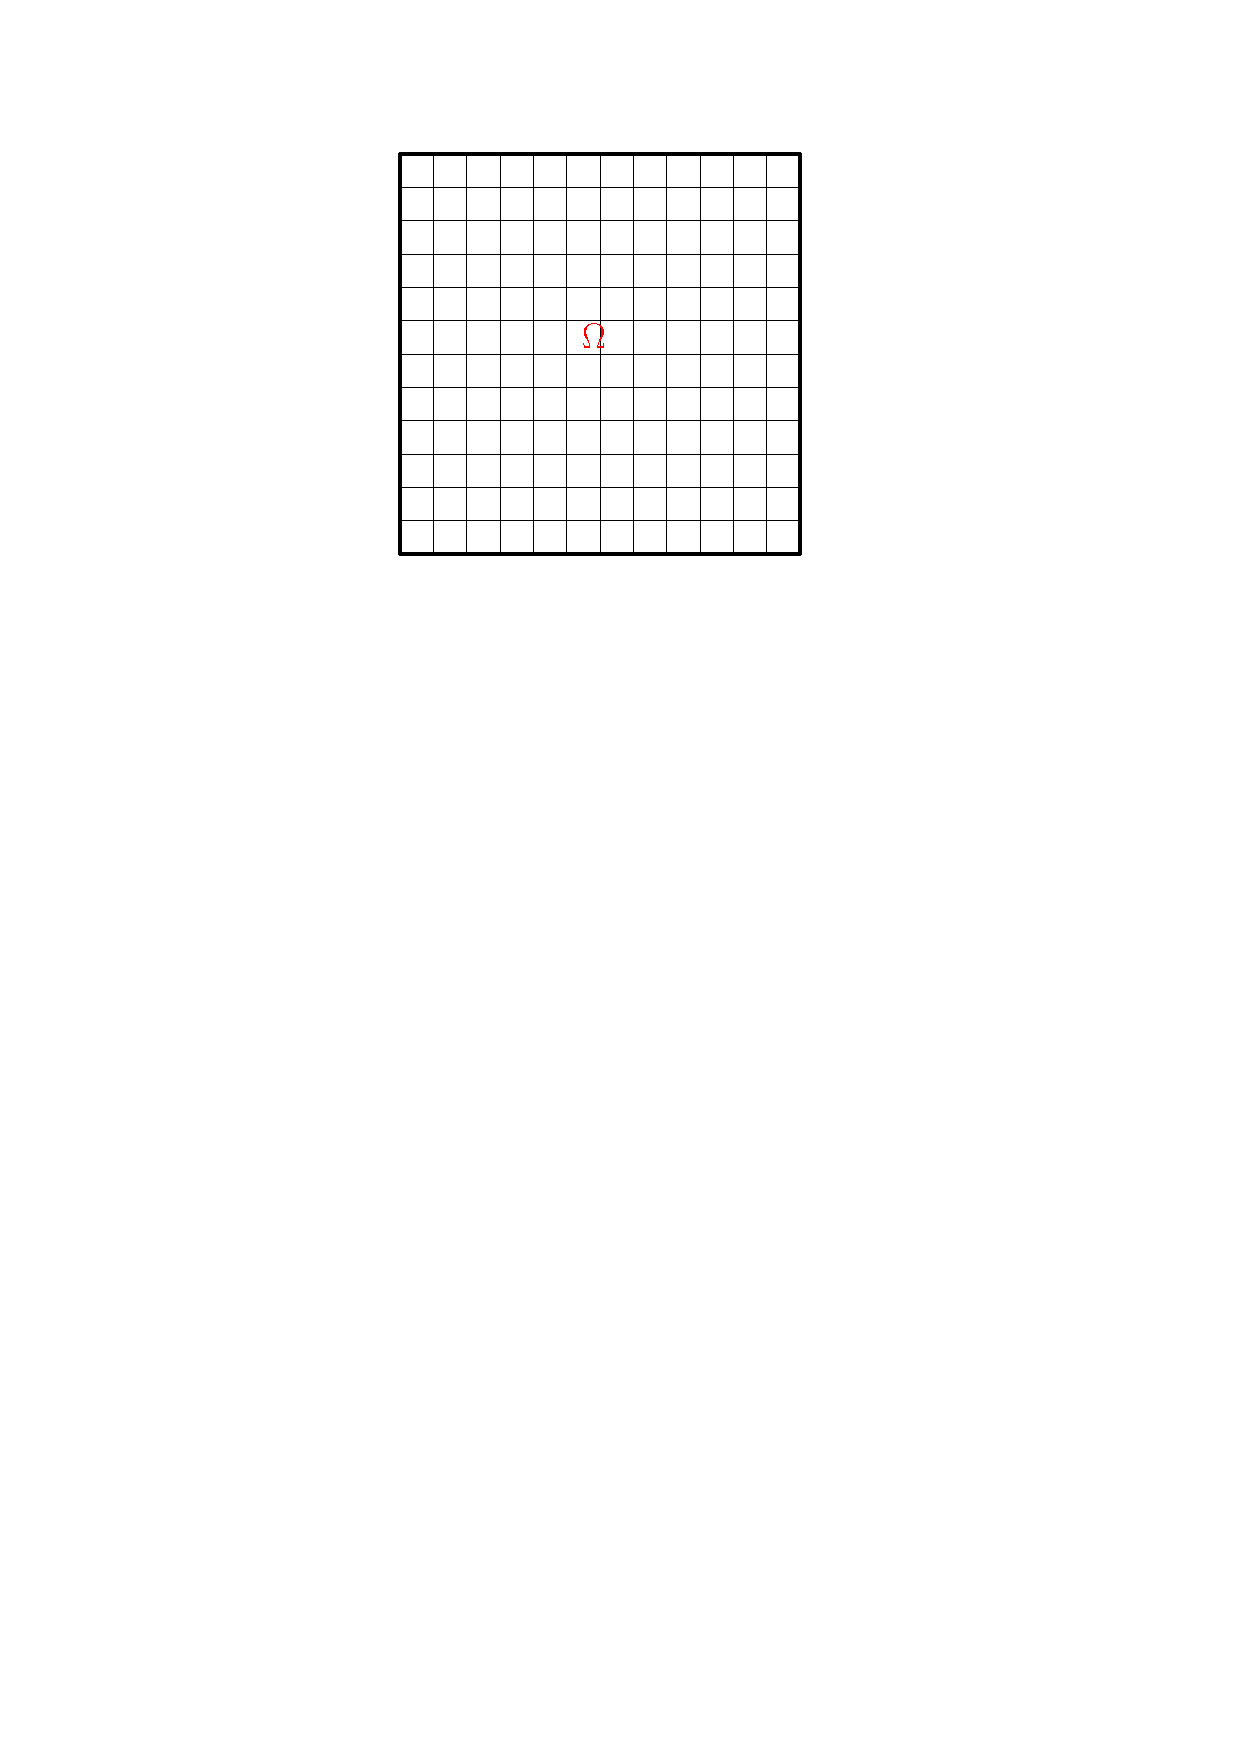
\includegraphics[width=0.5\textwidth]{./pics/domain.pdf}
	\end{tabular}
	\caption{\footnotesize The total computational domain.}\label{fig3: domain}
\end{figure}

\begin{enumerate}
	\item	Schur Complement \cite{duff1986direct} of problems on each subdomain  will eliminate all the interior unknowns and only retain the unknowns on the interface of . Denote the interface by .
	\item	Reduce the unknowns on the interface to construct the preconditioner.
	\item	Solve the linear system by using preconditioned conjugate gradient solver.
\end{enumerate}


\begin{figure}[h]
	\centering
	\begin{tabular}{c}
		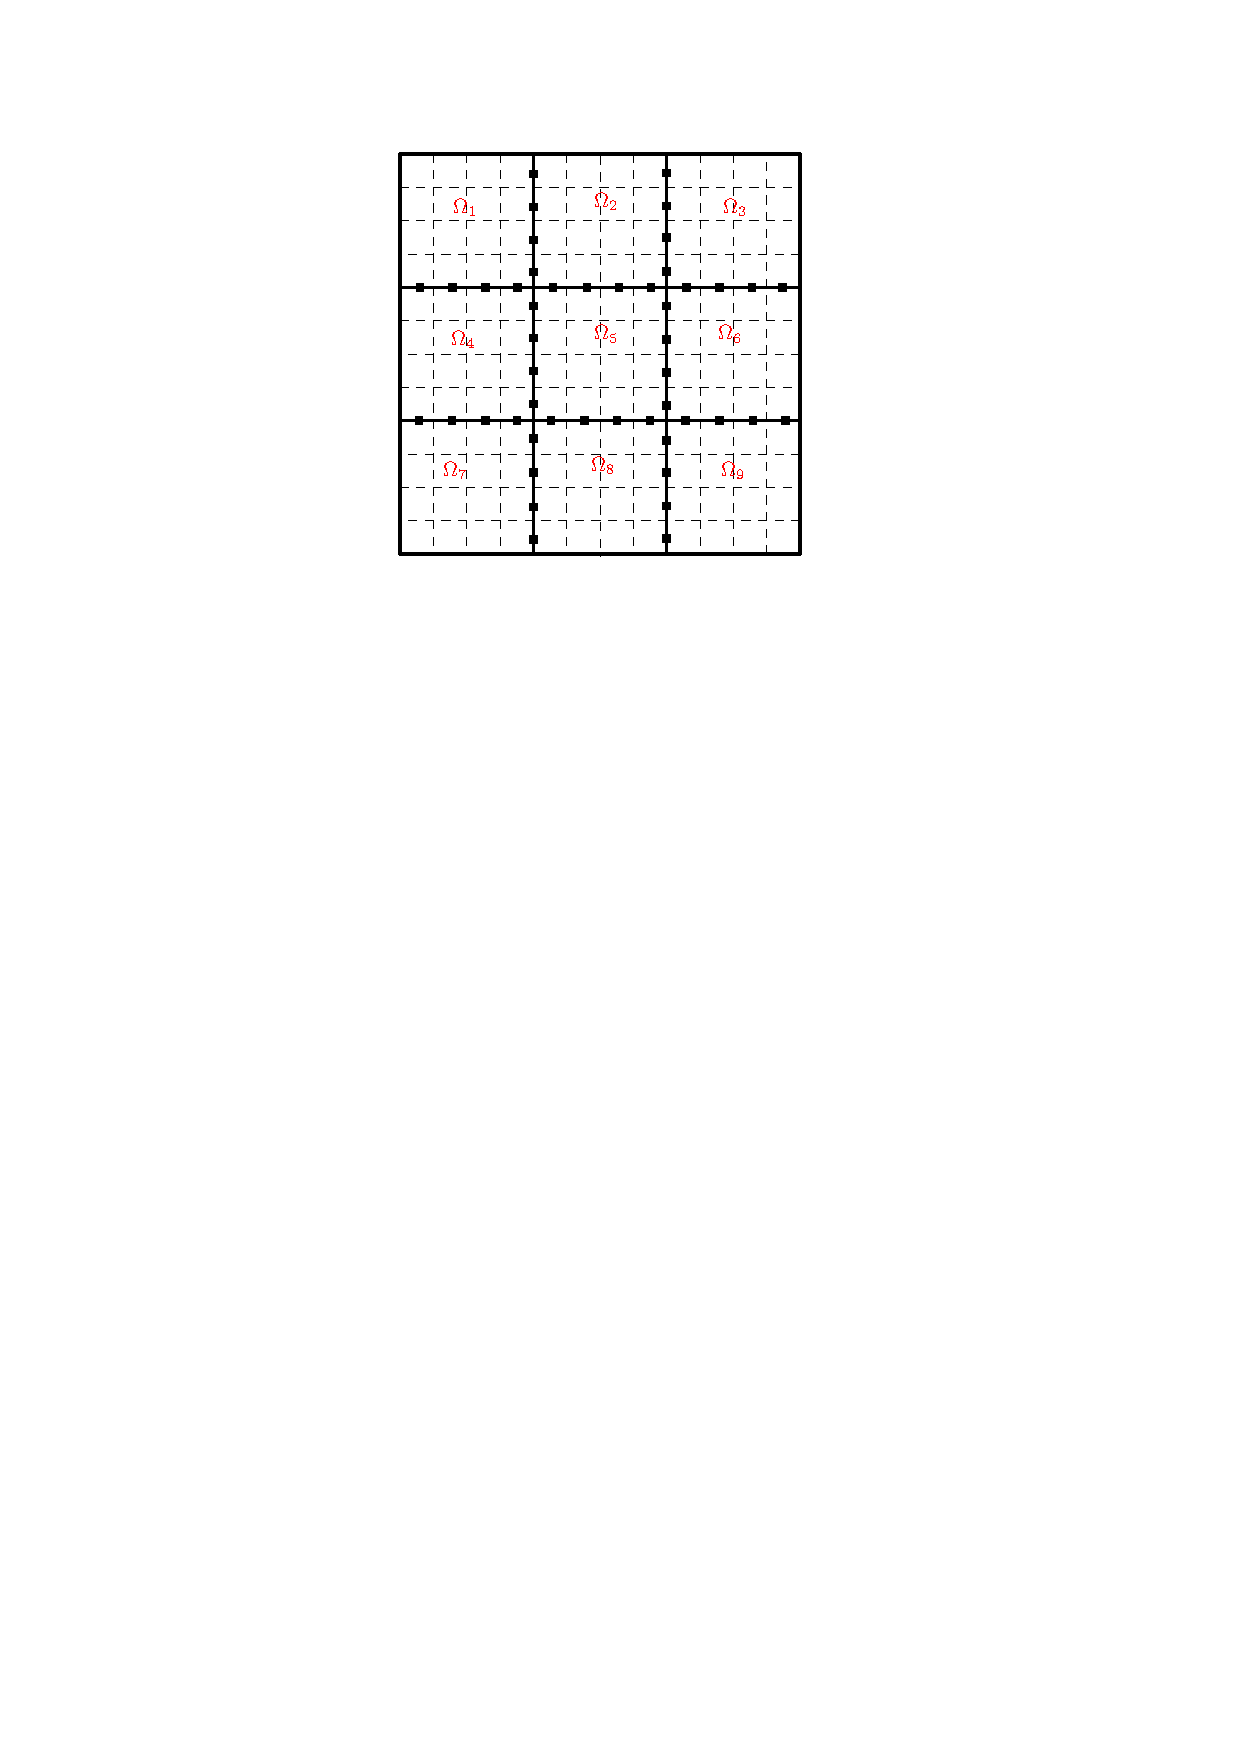
\includegraphics[width=0.6\textwidth]{./pics/domain2.pdf}
	\end{tabular}
	\caption{\footnotesize After the Schur complement method the computational domain becomes interior and interface.}\label{fig4: domain1}
\end{figure}

In the second step, the solid dot represents the unknown variables along the interface. They are shared by adjacent subdomains and should be calculated in the global matrix through Schur complement method. Even though the number of DOF in global matrix is drastically decreased, the communication overhead and scale of global matrix are still not satisfied the standard for high performance computing. In this way, we shall continuously split the interface into two spaces.


\begin{figure}[h]
	\centering
	\begin{tabular}{c}
		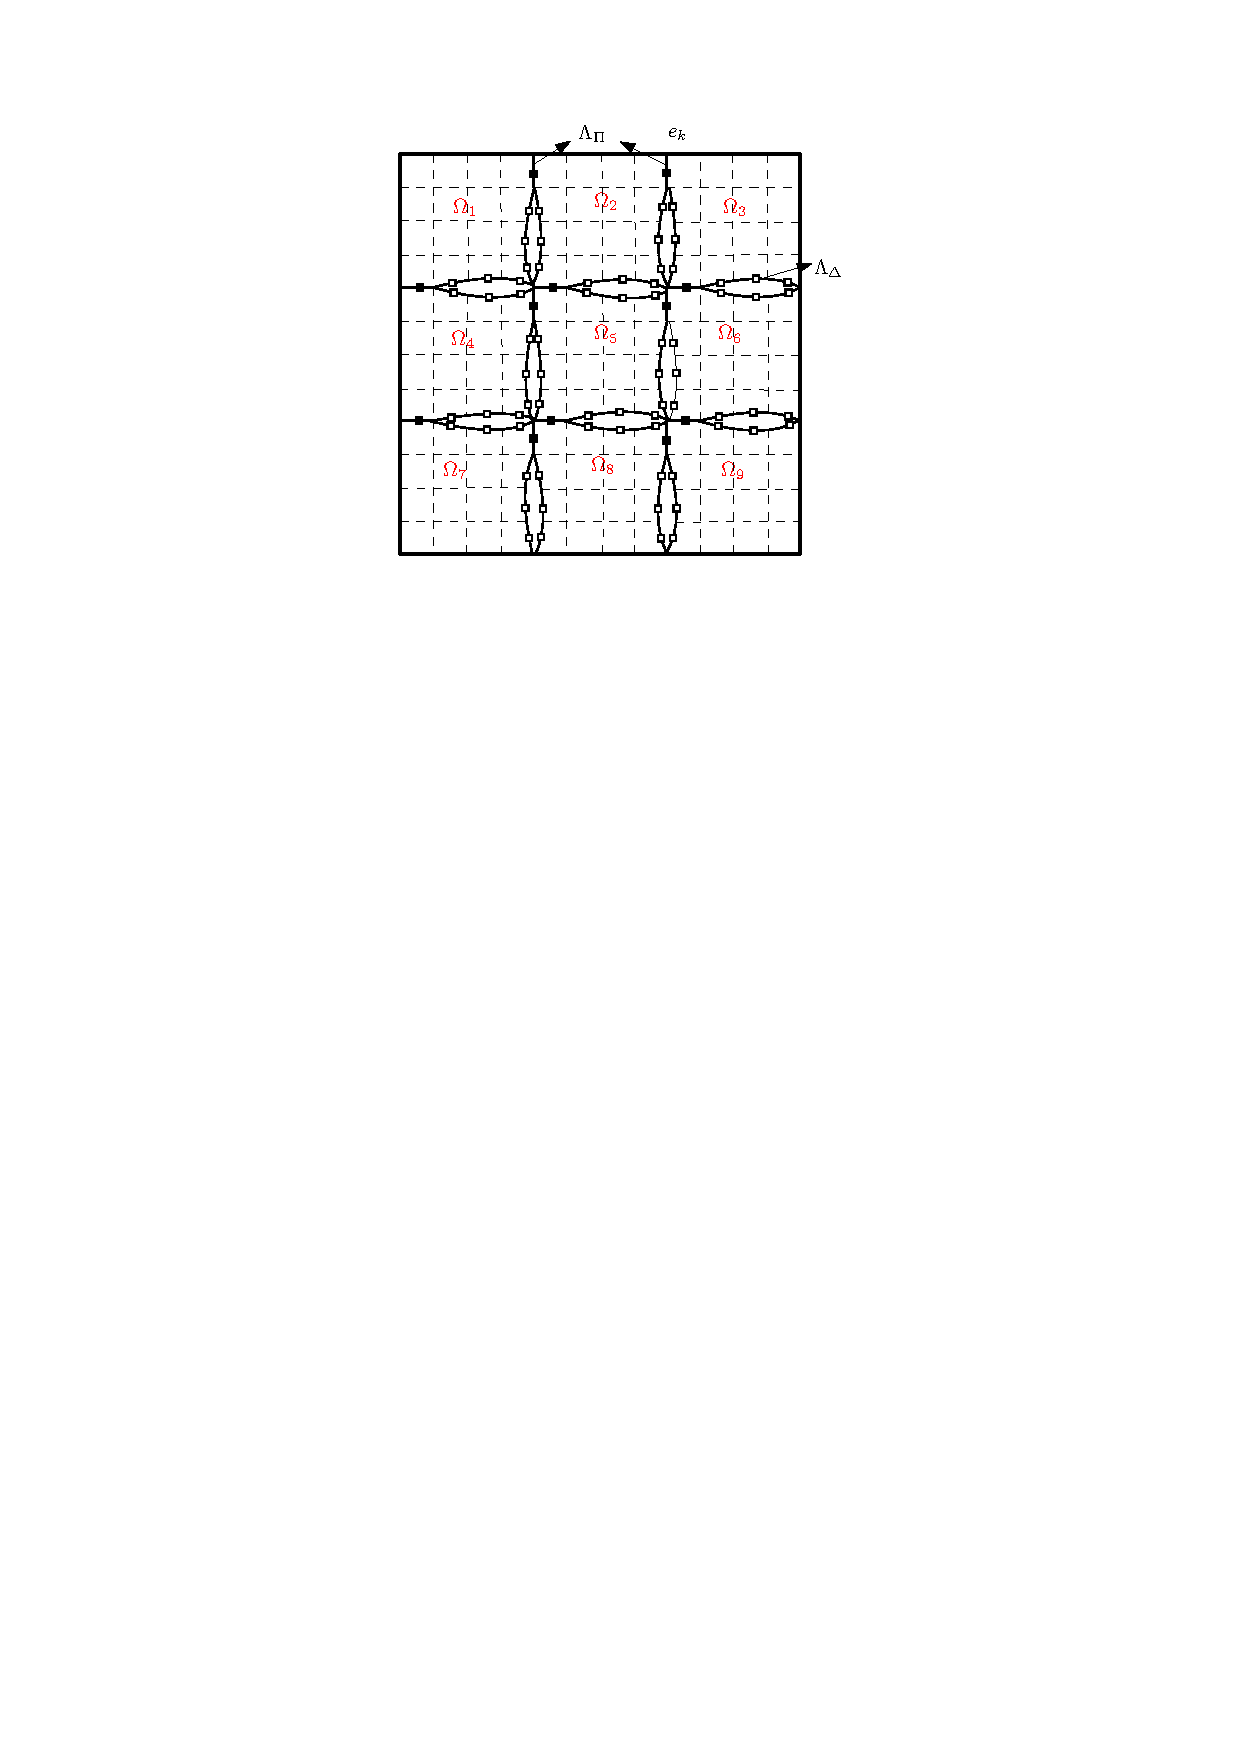
\includegraphics[width=0.6\textwidth]{./pics/domain3.pdf}
	\end{tabular}
	\caption{\footnotesize BDDC computational domain with only one cell boundary.}\label{fig5: domain2}
\end{figure}

In the third graph, we split the interface into primal and dual spaces. The circle represents the unknown variables belongs to dual space. They are calculated only in local matrices. We bridged the information from dual space to primal space through preconditioner. The remain dots are unknown variables in the primal spaces. They are the only information shall be communicated and calculated through MPI functions. Now the global matrix has been decreased to an optimal level which benefit us significantly in speedup test. 

One significant feature of this method is that when the number of subdomains increasing, the condition number of this method is bounded under the circumstance that an appropriate choice of the coarse DOFs and with regular subdomain shapes. The condition number grows only very slowly with the number of elements in each subdomain.

The number of iterations is also bounded in the same fashion. Meanwhile, the method scales well with the number of subdomains and size of the problem. 

\section{Schur Complement Method for subdomain $ \Omega_{j} $}

Denote the weak Galerkin solution on each subdomain $ \Omega_{j} $  For the consistency with Equation (1), we will use $ u_{h} $  to represent the weak Galerkin solution on each $ \Omega_{j} $.

To define the Schur complement system, the degrees of freedom $ u_h $  on each subdomain $ \Omega_j $ are partitioned into interior  $ u_{I}  $and interface $ u_{\Gamma} $ parts . Then, we can rewrite the unknown variable function as 
\begin{equation}
u_{h} = [u_{I0}, u_{Ib}, u_{\Gamma b}]
\end{equation}
and denote  $ u_I =  [u_{I0}, u_{Ib}]$, meanwhile, the $ u_{\Gamma} = u_{\Gamma b} $ . Consequently, the local Schur complements can be applied to each subdomain  in the following form
\begin{equation}
\begin{pmatrix}
A_{II} & A_{\Gamma I}^{T} \\
A_{\Gamma I} & A_{\Gamma \Gamma} \\
\end{pmatrix} \times
\begin{pmatrix}
u_{I} \\ u_{\Gamma}
\end{pmatrix}
\end{equation}

To define the Schur complement system, the DOFs on each subdomain are partitioned by interior and interface categories. Now the unknown function becomes $ u_{h} = [u_{I0}, u_{Ib}, u_{\Gamma b}] $, $ v_{h} = [v_{I0}, v_{Ib}, v_{\Gamma b}] $ and denote the interior unknown variable $ u_{i} = [u_{I0}, u_{Ib}] $ on the interface we have $ u_{\Gamma} = u_{\Gamma b} $ . For the assistant function the same rule applied to the assistant function $ v_I = [v_{I0}, v_{Ib}] $ , $ v_{\Gamma} = v_{\Gamma b} $ . The matrix form includes the assistant function should be following

\begin{equation}
\begin{pmatrix}
A_{II}^{u} & (A_{\Gamma I}^{u})^{T} & 0 & 0 \\
A_{\Gamma I}^{u} & A_{\Gamma \Gamma}^{u} & 0 & A_{\Gamma \Gamma}^{uv} \\
0 & 0 & A_{II}^{v} & (A_{\Gamma I}^{v})^{T} \\
0 & A_{\Gamma \Gamma}^{uv} & A_{\Gamma I}^{v} & A_{\Gamma \Gamma}^{v} 
\end{pmatrix} 
\begin{pmatrix}
u_{I} \\ u_{\Gamma} \\ v_{I} \\ v_{\Gamma}
\end{pmatrix}
\end{equation}
then we apply Schur complement method to eliminate the interior unknowns which will give the following equations

The interface stiffness matrix has the form as following
\begin{equation}
S_{\Gamma \Gamma}^{j} = A_{\Gamma \Gamma}^{(j)} - 
\begin{bmatrix}
A_{\Gamma I}^{(j)}
\end{bmatrix} \times
\begin{bmatrix}
A_{II}^{(j)}
\end{bmatrix}^{-1} \times
\begin{bmatrix}
A_{\Gamma I}^{(j)}
\end{bmatrix}^{T}
\end{equation}

The loading force along the interface has the form
\begin{equation}
f_{\Gamma}^{(j)} = b_{\Gamma}^{(j)} - 
\begin{bmatrix}
A_{\Gamma I}^(j) 
\end{bmatrix} \times
\begin{bmatrix}
A_{II}^{(j)}
\end{bmatrix}^{(-1)} \times
b_{I}^{(j)}
\end{equation}

Then denote the assembled matrix form
\begin{equation}
S_{\Gamma \Gamma} = \sum_{j = 1}^{N} {R_{\Gamma}^{(j)}}^{T} S_{\Gamma}^{(j)}R_{\Gamma}^{(j)}
\end{equation}
where $ R_{\Gamma}^{j} $ is the mapping vector to convert unknown variables between $ \Gamma $ global interface to $ \Gamma_i $ interfaces on subdomains $ \Omega_j $

Therefore, the global interface problem is constructed as 
\begin{equation}
S_{\Gamma \Gamma } \begin{pmatrix}
u_{\Gamma} \\ v_{\Gamma}
\end{pmatrix} = 
\begin{pmatrix}
f_{\Gamma}^{u} \\ f_{\Gamma}^{v}
\end{pmatrix}
\end{equation}

\section{BDDC Preconditioner}

Now, we eliminate most of the continuity across the interfaced, refers to Fig 5, and construct the BDDC preconditioner for the inverse of matrix $ S_{\Gamma} $.

In our BDDC formulation, the primal constraints are introduced over edges/faces. To define the BDDC preconditioner for the Schur complement problem, the interface space $ \Lambda_{\Gamma}^{(j)}s $ is a partitioned into two spaces dual, $ \Lambda_{\Delta}^{(j)} $  and primal, $ \Lambda_{\Pi}^{(j)} $. The dual space, $ \Lambda_{\Delta}^{(j)} $, corresponds to the subset of function in $ \Lambda_{\Gamma}^{(j)} $.

We define the partially assembled space as:
\begin{equation}
\hat{\Lambda}_{\Gamma} = \hat{\Lambda}_{\Pi} \oplus (\sum_{i = 1}^{N} \Lambda_{\Delta}^{(j)})
\end{equation}
where $ \hat{\Lambda}_{\Pi} $ is the assembled global primal space, single valued on $ \Gamma $, which is formed by assembling the local primal space, $ \Gamma_{\Pi}^{(j)} $. The BDDC preconditioner has been viewed as solving a finite element problem on partially assembled finite element space, $ \hat{\Lambda}_{\Gamma} $, to precondition the Schur complement problem whose solution lies in the fully assembled space $ \hat{\Lambda}_{\Gamma} $.

The key component of BDDC preconditioner \cite{eisenstat1981efficient}:
\begin{itemize}
	\item 	An averaging operator which restricts functions from $ \Lambda_{\Gamma} $  to $ \hat{\Lambda}_{\Gamma} $
	\item	A positive scaling factor $ \delta_{i}^{\dagger} (e_k) $ is defined for each interface $ e_k $ of the subdomain $ \Omega_j $ such that $ \delta_{i}^{\dagger} (e_k) + \delta_{j}^{\dagger}(e_{k}) = 1 $ where $ e_k = \partial \Omega_i \cap \partial \Omega_j$
	\item	Define $ D_{\Gamma}^{(i)} $ as the diagonal matrix formed by setting the diagonal entries corresponding to each nodal degree of freedom on $ e_k $ to $ \delta_{i}^{\dagger} (e_k) $
	\item	Define $ R_{D, \Gamma} : \hat{\Lambda}_{\Gamma} \rightarrow \Lambda_\Gamma$ as the product of $ R_{D, \Gamma} := D_{\Gamma} R_{\Gamma} $
\end{itemize}

The BDDC preconditioner has the following form that
\begin{equation}
M_{\Gamma_{BDDC}}^{-1} = R_{D, \Gamma}^{T} \tilde{S}_{\Gamma\Gamma}^{-1} R_{D, \Gamma}
\end{equation}

We interpret the above equation by using the unknown variable function $ u_{\Gamma} = [u_{r}, u_{c}]^{T} $ and the matrix can be written as
\begin{equation}
M = \begin{pmatrix}
S_{rr}^{(1)} & 0 & 0 & \cdots & 0 & S_{rc}^{(1)}\\
0 & S_{rr}^{(2)} & 0 & \cdots & 0 & S_{rc}^{(2)} \\
0 & 0 & S_{rr}^{(3)} & \cdots & 0 & S_{rc}^{(3)} \\
\vdots & \vdots & \vdots & \ddots & \vdots & \vdots \\
0 & 0 & 0 & \cdots & S_{rr}^{(N)} & S_{rc}^{(N)}\\
S_{cr}^{(1)} & S_{cr}^{(2)} & S_{cr}^{(3)} & \cdots & {S_{cr}^{(N)}} & S_{cc} \\
\end{pmatrix}
\end{equation}
the subscript $ c $ represents the unknown variables of constraints. The $ r $ represents the rest of unknown variables in computational subdomains.

The Lanczos matrix is applied to estimate the upper and lower eigenvalue bounds. The matrix is in a tridiagonal form and generated from the PCG iterations.

The BDDC method can be written as the form with preconditioner as
\begin{equation}
M_{\Gamma_{BDDC}}^{-1} S_{\Gamma \Gamma} u_{\Gamma} = M_{\Gamma_{BDDC}}^{-1} f_{\Gamma}
\end{equation}

\section{WG-BDDC Method Implementation}

In the Equaion (28), we can expand the constraints matrix as
\begin{equation}
S_{cc} = \sum_{i=1}^{N} A_{\Pi \Pi}^{(j)}
\end{equation}
meanwhile, the rest unknown variables matrix can be written in
\begin{equation}
S_{rr}^{(i)} = \begin{bmatrix}
A_{II}^{(j)} & A_{I \Delta}^(j) \\
A_{\Delta I}^{(j)} & A_{\Delta \Delta}^{(j)}\\
\end{bmatrix}
\end{equation}

The implementation of the WG-BDDC algorithm is presented as following:
\begin{equation}
\hat{R}_{D,\Gamma}^{T} \{ R_{\Gamma, \Delta}^{T} (\sum_{j = 1}^{N}\begin{bmatrix}
0 & {R_{\Delta}^{(j)}}^{T}
\end{bmatrix} \begin{bmatrix}
A_{II}^{(j)} & A_{I \Delta}^{(j)} \\
A_{\Delta I}^{(j)} & A_{\Delta \Delta}^{(j)}
\end{bmatrix}^{-1} \begin{bmatrix}
0 \\ R_{\Delta}^{(j)}\\
\end{bmatrix} )  R_{\Gamma \Delta} + \Phi S_{\Pi}^{-1} \Phi^{T}\} \hat{R}_{D, \Gamma}
\end{equation}
with
\begin{equation}
\Phi = R_{\Gamma\Pi}^{T} - R_{\Gamma \Delta}^{T} \sum_{j = 1}^{N} \begin{bmatrix}
0 & {R_{\Delta}^{(i)}}^{T} 
\end{bmatrix} \begin{bmatrix}
A_{II}^{(j)} & A_{I \Delta}^{(j)} \\
A_{\Delta I}^{(j)} & A_{\Delta \Delta}^{(j)}
\end{bmatrix}^{-1} \begin{bmatrix}
{A_{\Pi I}^{(j)}}^{T} \\ {A_{\Pi \Delta}^{(j)}}^{T} 
\end{bmatrix} R_{\Pi}^{(j)}
\end{equation}
and 
\begin{equation}
S_{\Pi} = \sum_{j = 1}^{N} {R_{\Pi}^{(j)}}^{T} \{ A_{\Pi \Pi}^{(j)} - \begin{bmatrix}
A_{\Pi I}^{(j)} & A_{\Pi \Delta}^{(j)}
\end{bmatrix}  \begin{bmatrix}
A_{II}^{(j)} & A_{I\Delta}^{(j)} \\
A_{\Delta I}^{(j)} & A_{\Delta \Delta}^{(j)}
\end{bmatrix}^{-1} \begin{bmatrix}
{A_{\Pi I}^{(j)}}^{T} & {A_{\Pi \Delta}^{(j)}}^{T}
\end{bmatrix} \} R_{\Pi}^{(j)}
\end{equation}
here the $ S_{\Pi} $ is the global coarse system matrix.

The preconditioned conjugate gradient is applied to solving above linear system. Theoretically, the condition number should be bounded as
\begin{equation}
\kappa (M_{\Gamma_{BDDC}}^{-1} \hat{S}_{\Gamma \Gamma}) \leq C (1 + log (\frac{kH}{h}))^{2}
\end{equation}
for a second order elliptic problem. The constant $ C $  is independent of solution order, $ p $, element size $ h $,  and the subdomain size $ H $ . Thus, the condition number and hence number of iteration required to converge are independent of the number of subdomains and only weakly dependent on the solution order and the size of subdomains.  

\section{Preconditioned Conjugate Gradient Method}
The conjugate gradient (CG) method is a well-known iterative method for solving large-scale symmetric and positive definite linear systems. The method is straightforward to implement and has the capability to handle complex domains and boundary conditions. 

The preconditioned conjugate gradient method has been reported by Bramble and Pasciak \cite{bramble1988preconditioning} to iteratively solving the symmetric saddle point problems. It inherits all great features of CG method and extends it to a higher level. This method is applied to a sparse system which is too large to handle by a direct method such as the Cholesky decomposition.

The details of PCG method is discussed by the following chart step by step. In terms of preconditioned, the major effort is to assemble the global preconditioner matrix. Then CG similar method is applied to solve the small global matrix. Thus, we can obtain the global corner solution with minimum overhead. Since both global and local matrices are sparse, the open source library LAPACK/BLAS \cite{anderson1999lapack} benefits the matrices calculation substantially.

The algorithm of PCG method is following:

\begin{algorithm}[H]
	\SetKwInOut{Input}{Input}
	\SetKwInOut{Output}{Output}
	
	% \underline{function Euclid} $(a,b)$\;
	\Input{$r_0:=b-Ax_0$\\
		$z_0:=M^{-1}r_0$\\
		$p_0:=z_0$\\
		$k\ :=0$}
	%\Output{$\gcd(a,b)$}
	\underline{Repeat} \;%$(a,b)$\;
	\begin{flalign*}
	\vspace{-20pt}
	\alpha_k:&=\frac{r_k^Tz_k}{p_k^TAp_k}&\\
	x_{k+1}:&=x_k+\alpha_kp_k\\
	r_{k+1}:&=r_k-\alpha_kAp_k
	\end{flalign*}
	\eIf{$r_k$ is sufficiently small}
	{
		return $x_{k+1}$\;
	}
	{
		\begin{flalign*}
		z_{k+1}:&=M^{-1}r_{k+1}&\\
		\beta_k:&=\frac{z_{k+1}^T r_{k+1} }{z_k^T r_k}\\
		p_{k+1}:&=z_{k+1}+\beta_kp_k\\
		k:&=k+1
		\end{flalign*}
	}
	\caption{Preconditioned Conjugate Gradient Algorithm}
\end{algorithm}

The condition number is calculated from Lanczos matrix. The global preconditioner matrix $ M $ is transfered into a tridiagonal matrix $ T_{mm} $. When the $ m $ is equal to the dimension of $ M $, $ T_{mm} $ is similar to $ M $. Then we calculate the eigenvalues of $ T_{mm} $ and obtain the condition number from calculating the ratio of  the maximum and minimum eigenvalue.

%======================================================

\section{Parallel Computing Scheme}

Message Passing Interface (MPI) \cite{gropp1996high} is portable and widely used as the communicator. We applied MPI to exchange the information between each non-overlapping subdomain. MPI provides a standard set of Fortran subprogram definitions. Intel MKL supports the modern MPI version which allows us to migrate the software on a variety of platforms. Besides, the MPI subprograms introduce the minimum overhead in both coding and testing stages.

The workflow of parallel computing scheme is following:
\begin{enumerate}
	\item	MPI communicator initiates work and distribute the parameters and mesh data to all the processors.
	\item	In every processor, the connectivity is analyzed and the local elemental matrices are constructed.
	\item	Through MPI subprograms, the local matrices are communicated and global preconditioner is constructed on every processor.
	\item	The global problem, whose size is significantly small, is calculated on every processor with PCG linear solver.
	\item	The global solution is reduced to each processor for the local solution recovery. 
\end{enumerate}

\begin{figure}[h]
	\centering
	\begin{tabular}{c}
		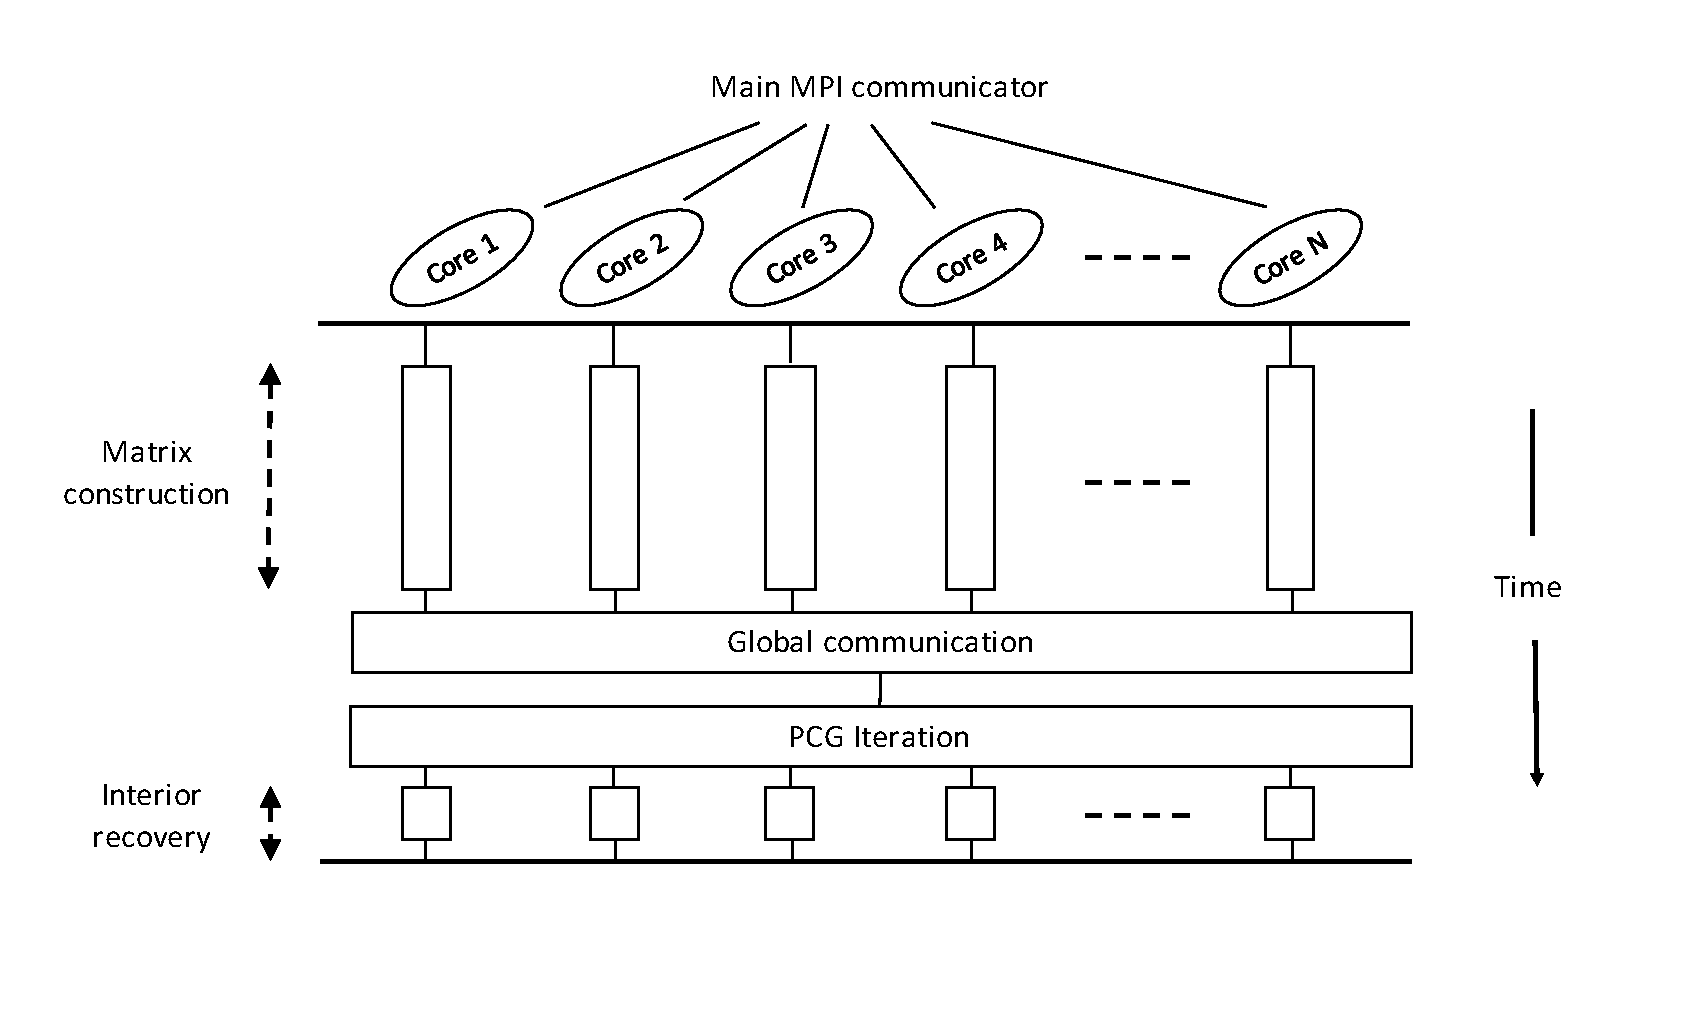
\includegraphics[width=1.0\textwidth]{./pics/mpi_flow.eps}
	\end{tabular}
	\caption{\footnotesize Parallel computing work flow.}\label{fig6: mpi}
\end{figure}
The software has been tested on the George Washington University cluster, ColonialOne, with Xeon E5-2650v2 2.6 GHz 8-core processors with 128 GB of RAM each.

%=================================================
\section{Numerical Results}

\subsection{Poisson Equation}
The WG element can choose different order of basis function in weak gradient equation. Hence, we test the combination order of interior, boundary and weak gradient shape functions. 

The Poisson equation $ -\nabla \cdot (\nabla \mathbf{u}) = \mathbf{f} $ is considered in the test. Let $ \Omega = (0, 1) \times (0, 1) $, $ a = I $, and $ f $ are chosen such that the exact solution is $ u = sin(\pi x) sin(\pi y) $

We choose different weak Galerkin elements for validating our WG-BDDC numerical scheme. The unit square is firstly decomposed into $ N \times N $ subdomains as the coarse mesh with length $ H = 1 / N $. In every subdomain, all elements are further triangulated into a $ 2 n \times n $ triangles, and the finite mesh has the size $ h = 1/(N\times n) $. The preconditioned system is solved by the PCG solver. In every iteration, the $ L^2- $norm of the residual is reduced by a factor of $ 10^{-6} $. The $ L^{2} $ error is calculated by using the equation $ e_{L^{2}} = \sqrt{\sum_{k = 1}^{n} (u - u_{t})^{2} } $

\begin{table}[h]
	\setlength{\tabcolsep}{2pt} {
		\caption{ Performance with $P_{k}P_{k-1}P_{k-1}^2$.}
		\label{Tab:case1_PkPk-1Pk-1}
		\vspace{-5pt}
		\begin{center}
			%	\scalebox{0.6}{
			\begin{tabular}{c|cccc|c|cccc}
				\hline
				\multirow{2}{*}{\#sub} &\multicolumn{4}{c|}{$k=1$ and $H/h=8$} &\multirow{2}{*}{$H/h$} &\multicolumn{4}{c}{$k=1$ and \#sub=64}\\ 
				& Cond.   & Iter. &$L^2$-error & $ O $ & & Cond.   & Iter. &$L^2$-error &$ O $ \\
				\hline
				$4\times 4$     &2.217 &5 &1.6013e-3 &- &4   &1.722 &7   &1.6013e-3 & -\\
				$8\times 8$     &2.390 &9 &3.9939e-4 & 2.0 &8   &2.390 &9   &3.9939e-4& 2.0\\
				$16\times 16$ &2.335 &8 &9.9789e-5 & 2.0 &16 &3.245 &10 &9.9789e-5 & 2.0\\
				$32\times 32$ &2.325 &8 &2.4944e-5 & 2.0 &32 &4.239 &11 &2.4944e-5 & 2.0 \\
				\hline
				\multirow{2}{*}{\#sub} &\multicolumn{4}{c|}{$k=2$ and $H/h=8$} &\multirow{2}{*}{$H/h$} &\multicolumn{4}{c}{$k=2$ and \#sub=64}\\ 
				& Cond.   & Iter. &$L^2$-error & $ O $ & & Cond.   & Iter. &$L^2$-error & $ O $  \\
				\hline
				$4\times 4$    &3.528 & 8  &7.1456e-5 & -  &4   &2.900 &10 &7.1456e-5 & - \\
				$8\times 8$    &3.803 &10 &8.9214e-6 & 3.0 &8   &3.803 &10 &8.9214e-6 & 3.0 \\
				$16\times 16$&3.768 &10 &1.1150e-6 & 3.0 &16 &4.957 &12 &1.1150e-6 & 3.0 \\
				$32\times 32$&3.758 &10 &1.3938e-7 & 3.0 &32 &6.218 &13 &1.3938e-7 & 3.0\\
				\hline
			\end{tabular}
			%	}
		\end{center} }
	\end{table}
	
	The first test is implemented for weak Galerkin element $ u_0 \in P_k, u_b \in P_{k - 1} $, and $ \nabla_w u \in P_{k - 1} $. \ref{Tab:case1_PkPk-1Pk-1} shows the condition number of lanczos matrix and the iteration number in PCG solver. From the \ref{Tab:case1_PkPk-1Pk-1}, we can see that the condition number is independent of the number of subdomain, while it depends on $ H/h $ as $ (1 + log(\frac{H}{h}))^{2} $. Meanwhile, the communication between each adjacent subdomain does not introduce any error to the results. With the increasing of number of subdomains, we obtain stable second and third order of results. The iteration number of global matrix increases slowly to the number of subdomains.
	
	
	\begin{table}[h]
		\small
		\setlength{\tabcolsep}{1pt} {
			\caption{ Performance with $P_{k}P_{k}P_{k-1}^2$.}
			\label{Tab:case1_PkPkPk-1}
			\begin{center}
				%\scalebox{0.8}{
				\begin{tabular}{c|cccc|c|cccc}
					\hline
					\multirow{2}{*}{\#sub} &\multicolumn{4}{c|}{$k=1$ and $H/h=8$} &\multirow{2}{*}{$H/h$} &\multicolumn{4}{c}{$k=1$ and \#sub=64}\\ 
					& Cond.   & Iter. &$L^2$-error & $O1$ & & Cond.   & Iter. &$L^2$-error & $O$\\
					\hline
					$4\times 4$ & 2.451 & 7 & 1.0109e-3 & - &$4$ &1.968 &8 &1.0109e-3 &-\\
					$8\times 8$ &2.648 &9 &2.5117e-4 &	2.0  &8 &2.648 &9 &2.5117e-4 &2.0 \\
					$16\times 16$ &2.629 &9 &	6.2696e-5 &2.0  &16 &3.529 &10 &6.2696e-5 &2.0\\
					$32\times 32$ &2.617 &9 &1.5668e-5 &2.0  &32 &4.619 &12 &1.5668e-5 &2.0\\
					\hline
					\multirow{2}{*}{\#sub} &\multicolumn{4}{c|}{$k=2$ and $H/h=8$} &\multirow{2}{*}{$H/h$} &\multicolumn{4}{c}{$k=2$ and \#sub=64}\\ 
					& Cond.   & Iter. &$L^2$-error &  $\lambda_1$ & & Cond.   & Iter. &$L^2$-error & $\lambda_1$\\
					\hline
					$4\times 4$ & 3.805 &8 &6.6333e-5  &- &4 &3.926 &11 &6.6333e-5  &-\\
					$8\times 8$ & 4.003 &12 &8.2709e-6  & 3.0 &8 &4.003 &12 &8.2709e-6  &3.0 \\
					$16\times 16$ &3.943 &12 &1.0334e-6  &3.0 &16 &5.084 &13 &1.0334e-6  &3.0\\
					$32\times 32$ &3.917 &12 &1.2917e-7  &3.0 &32 &6.329 &13 &1.2918e-7  &3.0\\
					\hline
				\end{tabular}
				%	}
			\end{center} }
		\end{table}
		
		The second test is the weak Galerkin element with order $ u_{0} \in P_{k} $, $ u_{b} \in P_{k} $ and $ \nabla_{w} \in P_{k - 1} $. The condition number has the identical pattern of the theoretical convergence rate. Comparing with the first example, we can find the convergence rates and accuracy have optimal agreement to the degree of polynomial in $ u_{0} $. The parallel scalability is up to 1,000 processors.
		
		\begin{table}[h]
			\small
			\vspace{-10pt}
			\setlength{\tabcolsep}{1pt} {
				\caption{Case 1: Performance with $P_{k}P_{k}P_{k}^2$.}
				\label{Tab:case1_PkPkPk}
				\vspace{-5pt}
				\begin{center}
					%\scalebox{0.8}{
					\begin{tabular}{c|cccc|c|cccc}
						\hline
						\multirow{2}{*}{\#sub} &\multicolumn{4}{c|}{$k=1$ and $H/h=8$} &\multirow{2}{*}{$H/h$} &\multicolumn{4}{c}{$k=1$ and \#sub=64}\\ 
						& Cond.   & Iter. &$L^2$-error & $O$  & & Cond.   & Iter. &$L^2$-error & $O$ \\
						\hline
						$4\times 4$     &3.671 & 8  &2.1451e-4 &- &4   &3.024 &10 &2.1451e-4 &- \\
						$8\times 8$     &3.965 &10 &5.2129e-5 &2.0  &8   &3.965 &10 &5.2129e-5 &2.0 \\
						$16\times 16$ &3.934 &10 &1.2937e-5 &2.0  &16 &5.153 &12 &1.2937e-5 &2.0 \\
						$32\times 32$ &3.922 &10 &3.2281e-6 &2.0  &32 &6.472 &14 &3.2281e-6 &2.0 \\
						\hline	
						\multirow{2}{*}{\#sub} &\multicolumn{4}{c|}{$k=2$ and $H/h=8$} &\multirow{2}{*}{$H/h$} &\multicolumn{4}{c}{$k=2$ and \#sub=64}\\ 
						& Cond.   & Iter. &$L^2$-error & $O$ & & Cond.   & Iter. &$L^2$-error & $O$ \\
						\hline
						$4\times 4$     &4.620 &8   &6.7627e-6 &-  & 4  &3.859 &11 &6.7628e-6 &- \\
						$8\times 8$     &4.987 &12 &7.8998e-7 &3.0  &8   &4.987 &12 &7.8998e-7 &3.0 \\
						$16\times 16$ &4.921 &12 &9.6925e-8 &3.0  &16 &6.235 &13 &9.6931e-8 &3.0 \\
						$32\times 32$ &4.901 &12 &1.2058e-8 &3.0  &32 &7.673 &15 &1.2060e-8 &3.0 \\
						\hline
					\end{tabular}
					%}
				\end{center} }
			\end{table}
			
			In the third test, we implement the weak Galerkin element $ u_{0} \in P_{k} $, $ u_{b} \in P_{k} $ and $ \nabla_{w} u \in P_{k} $. The $ P_k P_k P_k^2 $ element deliveries the most accurate result among all three types of element. The reason is that all three shape functions of interior variable, boundary variable and weak gradient have the same order. 
			
			
			\subsection{Linear Elastic Equation}
			
			We consider the linear elastic equation (1) in the square domain $ \Omega = (0, 1)^{2} $ which is decomposed into uniform square subdomains with size $ H $. For each subdomain, it is partitioned into uniform quadrilateral mesh with size $ h $. The exact solution is given by
			\begin{equation}
			u = \begin{pmatrix}
			sin(2\pi x)sin(2\pi y) \\ 1
			\end{pmatrix}
			\end{equation}
			
			\begin{table}[h]
				\small
				\vspace{-10pt}
				\setlength{\tabcolsep}{1pt} {
					\caption{Case 1: Performance with $P_{1}P_{1}$, $ \lambda = 1, \mu = 0.5 $}
					\label{Tab:case1_PkPkPk linear}
					\vspace{-5pt}
					\begin{center}
						%\scalebox{0.8}{
						\begin{tabular}{c|cccc|c|cccc}
							\hline
							\multirow{2}{*}{\#sub} &\multicolumn{4}{c|}{ $H/h=8$} &\multirow{2}{*}{$H/h$} &\multicolumn{4}{c}{$k=1$ and \#sub=64}\\ 
							& Cond.   & Iter. &$L_{Max}$-error & $O$& & Cond.   & Iter. &$L^2$-error & $O$ \\
							
							\hline
							$2\times 2$     & 2.281 & 8   & 8.484e-2 & - & 4   & 2.212 &11 & 2.993e-1 &- \\
							$4\times 4$     &3.922 &12 &2.1787e-2 & 1.96 & 8   & 3.069 &12 & 8.567e-2 & 1.9  \\
							$8\times 8$  & 4.895 &17 &5.4706e-3 & 1.99 & 16   & 4.143 &13 & 2.217e-2 & 2.0 \\
							$16\times 16$ &5.238&17 &1.3675e-3 & 2.00 & 32   & 5.437 &15 & 5.575e-3 & 2.0 \\
							\hline	
						\end{tabular}
						%	}
					\end{center} }
				\end{table}
				
				We test the performance of WG-BDDC on cluster and present the speedup figure which indicates the superlinear acceleration and good scalability. 
				
				\begin{figure}[h]
					\centering
					\begin{tabular}{cc}
						\includegraphics[width=0.6\textwidth]{./pics/p1time.eps} 
					\end{tabular}
					\caption{\footnotesize The running time .vs. number of processors.}\label{fig6: time}
				\end{figure}
				
				
					\begin{figure}[h]
						\centering
						\begin{tabular}{cc}
							 \includegraphics[width=0.6\textwidth]{./pics/p1speed.eps}
						\end{tabular}
						\caption{\footnotesize The speedup .vs. number of processors.}\label{fig6: time}
					\end{figure}
				
				The blue dot line called WGDD represents WG-BDDC method. we can see from the above figures that the superlinear speedup is captured within the increasing of the number of subdomains. The main concern for BDDC method is that the balance between global matrix, the preconditioner, and the local matrices. It is important to estimate the size of preconditioner and choose proper number of processors.
				
				
	we report a novel parallel computing method. This method integrated the newly developed weak Galerkin finite element method with balancing domain decomposition with constraints. The MPI library is set up for information communication between each processor. The optimal convergence rate and promising scalability of this WG-BDDC method are observed.
	
	To this method, it is convenient to implement high order element. We have multiple choices on interior, boundary and gradient basis functions which is an obvious flexibility to numerical calculation. We can design the element type based on our need. From the optimal convergence rate, we can conclude that this method is robust and highly compatible to different element orders.
	
	For the results, all test cases have well bounded condition numbers for the global matrices which fits our initial assumption properly. Meanwhile, the superlinear feature from the speedup graph is also in favor of high performance computing. This is the first attempt to introduce weak Galerkin to engineering purpose implementation. The optimal performance on parallel computing indicates a promising future of this method.